Sau khi hoàn thành khóa luận này, tác giả đã có thêm những kiến thức, kinh nghiệm như:
\begin{itemize}
    \item Cách tìm, đọc, nghiên cứu tài liệu.
    
    \item Tổ chức, làm việc của 1 nhóm nghiên cứu.
    \item Hiểu biết thêm và thiết kế và lập trình mạch.

    \item Kinh nghiệm trong lập trình phần mềm.
    \item Kiến thức cơ bản về học máy.v.	Kiến thức cơ bản về học máy.
    \item Ứng dụng vào công việc hiện tại.
\end{itemize}
Tuy nhiên đây mới chỉ là những bước đầu khai phá những kiến thức mới trong một định hướng nghiên cứu đòi hỏi sự hợp tác của nhiều ngành đặc biệt là ngành y học. Qua những điều đã đạt được, tác giả và nhóm nghiên cứu sẽ dần dần đúc rút thêm nhiều kinh nghiệm, kiến thức và kỹ năng để sớm hoàn thiện mục tiêu trong thời gian tới.

\textbf{Hướng phát triển trong thời gian tới}

Đây là những tìm hiểu bước đầu của tác giả về thiết bị chẩn đoán chứng ngưng thở khi ngủ OSA vì vậy còn nhiều hạn chế về phần cứng và phần mềm. Hiện nay tác giả mới chỉ đánh giá các tư thế ngủ thông qua các ngưỡng của dữ liệu của 3 trục cảm biến. Điều này khiến việc trả về kết quả có thể chưa đạt độ chính xác cao. Vì vậy tác giả đã tìm hiểu các mô hình học máy để đánh giá 1 cách chính xác. Hơn nữa việc bật màn hình điện thoại liên tục cũng làm hạn chế trải nghiệm của người dùng. Tác giả đã có những ý tưởng để cải thiện hiệu năng và dễ thao tác hơn đó với ứng dụng trên điện thoại. Đó là tích hợp them module wifi trên phần cứng từ đó tác giả đẩy dữ liệu trực tiếp lên phía server. Sau đó thiết bị trên điện thoại sẽ theo dõi trực tiếp từ server rồi hiển thị thông qua các ứng dụng chạy ngầm (foreground service android). Điều này có thể giúp người dùng trách bật ứng dụng liên tục nhưng cũng khiến thời lượng pin của thiết bị giảm xuống.
Như đã đề cập ở chương 2 tương lai tác giả sẽ có định hướng áp dụng các mô hình học máy cho đánh giá tư thế ngủ hơn nữa là đánh giá chỉ số AHI dựa trên các thông số thu nhận từ các cảm biến. Tác giả cũng tìm hiểu nhiều cách để lấy được bộ dữ liệu và đánh nhãn thì chủ yếu các tác giả đánh nhãn bằng phương pháp thủ công như dùng máy ảnh để ghi lại, hoặc lấy nhãn của 1 hành động trong 1 thời gian cố định hoặc đánh trực tiếp trên thiết bị di động. Từ đó tác giả sẽ lên ý tưởng thiết kế tích hợp nút bấm trên ứng dụng điện thoại phục vụ việc lấy nhãn cho tập dữ liệu.
Về phía phần mạch, nhóm tác giả đang phát triển và có những bước vẽ trên phần mềm Altium.

\begin{figure}
    \centering
    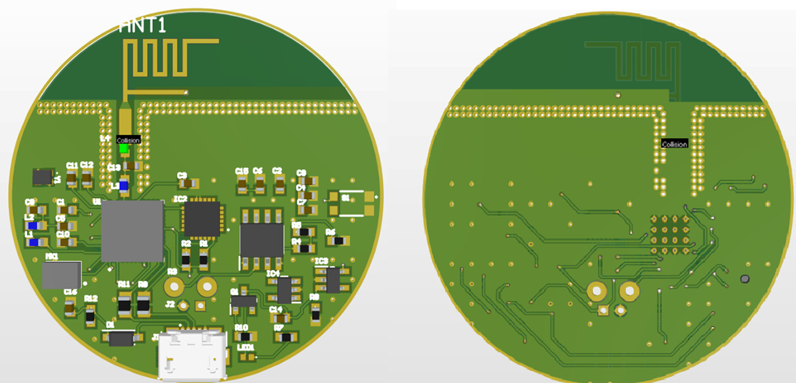
\includegraphics[width=0.75\linewidth]{images/macjh.png}
    \caption{Mạch thiết kế trên phần mềm Altium}
    \label{macjh}
\end{figure}

Trong thời gian tương lại, tác giả sẽ hoàn thành mạch in và thử nghiệm trên đó.
Mục tiêu cuối cùng là ứng dụng được sản phẩm vào thực tiễn để có thêm cơ sở giúp các bác sĩ chẩn đoán sớm được những bệnh nhân mắc chứng OSA. Để hoàn thành được mục tiêu đó, trong tương lai, cả nhóm cần hoàn thiện các vấn đề còn tồn đọng và phát triển thêm những tính năng mới. Vấn đề áp dụng các mô hình học máy sẽ được nhóm tác giả tiếp tục phát triển không chỉ dừng lại ở đánh giá tư thế ngủ mà còn đánh giá chỉ số AHI.
